\documentclass[a4paper, 12pt]{scrreprt}

\usepackage[utf8]{inputenc}

\usepackage{float}
\usepackage{longtable}
\usepackage{graphicx}
\usepackage{hyperref}
\usepackage{xcolor}
\usepackage{caption}
\usepackage{parskip}
\usepackage[onehalfspacing]{setspace}
\usepackage{chngcntr}
\usepackage[
backend=biber,
sorting=none,
citestyle=authoryear,
natbib=true
]{biblatex}
\usepackage[ngerman]{babel}
\usepackage{enumitem}


\setlist[enumerate]{label*=\arabic*.}
\addbibresource{references.bib}
\hypersetup{
	colorlinks,
	linkcolor={black},
	citecolor={black},
	urlcolor={black}
}
\defbibfilter{bookInbook}{
	type=book or
	type=inbook
}
\graphicspath{ {./img/} }

\counterwithout{figure}{chapter}
\counterwithout{table}{chapter}

\newcommand\klammercite[1]{%
	(\citealt{#1})}

\parskip 1.75ex plus 0.5ex minus 0.5ex

\title{Platzhalter Titel}
\subtitle{}
\author{Lennart Ploog}
\publishers{IS Medieninformatik\\ Fakultät 4\\ Hochschule Bremen}

\makeatletter
\let\inserttitle\@title
\makeatother

\begin{document}
	\maketitle
	\newpage
	\tableofcontents
	\newpage
\chapter{Abstract}
TODO: Acronyms, Figures
\chapter{Einleitung}
\section{Problemfeld}
Ob auf Reisen, im Supermarkt oder im Fahrstuhl -- Situationen, in denen mobile Endgeräte keine stabile Internetverbindung haben, kommen im Alltag häufiger vor als gewünscht. In vielen Entwicklungsländern und auch in ländlichen Gegenden entwickelter Industriestaaten fehlt dafür gar die komplette Infrastruktur. Im Laufe der letzten Jahre eröffneten Innovationen im Bereich der Browser-Technologien, allen voran der Service-Worker, neue Möglichkeiten für die Webentwicklung. Als Offline-First-Applikationen werden Webanwendungen bezeichnet, die ihre Funktionalität so weit es geht behalten, wenn die Verbindung zum Internet getrennt ist.

Eine der Kernherausforderungen der Entwicklung von Offline-First Applikationen ist die Synchronisation von Daten. Werden offline Änderungen vorgenommen, sollen diese nicht verloren gehen. Hat sich der Zustand der Applikation, beispielsweise durch Modifikationen eines anderen Nutzers, in der Zwischenzeit jedoch geändert, müssen beide Änderungen zusammengebracht, also synchronisiert werden. Der Prozess der Synchronisation ist oft aufwendig, denn zum Einen muss ermittelt werden, wo sich beide Replikationen unterscheiden und zum Anderen muss vermieden werden, dass die Änderungen sich in die Quere kommen. 

Gängige Lösungen zu einer solchen Zusammenführung von Daten umfassen die Nutzung bestimmter Datenbanken-Technologien. Dazu gehören Datenbanken mit implementierter Synchronisation wie CloudDB oder auch Backend-as-a-Service Produkte wie Firebase oder IBM Cloudant, welche ebenfalls eine solche Funktionalität anbieten. Um dies zu vermeiden, verzichten viele Applikationen bei Konflikten auf eine Synchronisation und einer der beiden Nutzer verliert seine vollbrachte Arbeit.

\section{Ziel der Arbeit} 

Ziel dieser Arbeit ist es, eine Lösung zur Synchronisation von Daten in Offline-First Anwendungen mit Hilfe von konfliktfreien replizierten Datentypen, kurz CRDTs, umzusetzen. Der Einsatz von CRDTs ermöglicht, dass Daten in einem verteilten System in beliebiger Reihenfolge ausgetauscht werden können und dennoch zum gleichen Zustand aller Replikationen führen. Durch die Implementierung einer Datenstruktur, welche auf CRDTs aufbaut, kann der Prozess der Synchronisierung somit vermieden werden. Diese Lösung soll unabhängig von der gewählten Datenbank sein.

So ergeben sich folgende Forschungsfragen:

\begin{itemize}
	\item Wie können CRDTs in Offline-First Applikationen verwendet werden?
	\item Welche CRDTs bieten sich zur Umsetzung von Offline-First Applikationen an und wie werden diese in die Datenbanken (Client und Server) implementiert?
	\item Welche Vor- und Nachteile bietet die Nutzung von CRDTs im Vergleich zu anderen Optionen zur Synchronisierung von Daten in Offline-First Applikationen.
\end{itemize}

\section{Vorgehen}

Es gibt verschiedene Möglichkeiten, wie CRDTs in Webapplikationen eingesetzt werden können. Bevor die Implementation der Datenstruktur beginnen kann, muss ermittelt werden, welche CRDTs sich am besten für die Daten des Prototypen eignen. Um dies herauszufinden eignet sich die Recherche in den im Abschnitt Verwandte Arbeiten erwähnten Publikationen. Darüber hinaus lohnt es sich an dieser Stelle auch in Erfahrung zu bringen, welche CRDTs bis heute in fertigen Applikationen verwendet wurden. Auch Literatur zum Austausch von Daten in Applikationen zu kollaborativem Editieren zu P2P Netzwerken bietet sich zur Recherche an, denn in diesen Bereichen sind CRDTs schon weiter verbreitet als in anderen Anwendungsgebieten.

Damit der Prototyp als praxisnahes Beispiel dienen kann, sollte auch der Stand der Technik im Themenbereich der Offline-First Anwendungen ermittelt werden. Um einzuordnen, an welcher Ebene der Architektur der Applikation sich die umzusetzende Funktionalität zur Zusammenführung der Daten am besten einbauen lässt, lohnt sich auch ein Blick auf bestehende Lösungen, welche die Synchronisation nicht direkt auf der Datenbankebene durchführen, sondern zwischen Applikation und Datenbank.

\subsection{Prototyp}
Platzhalter, genauer nach Fertigstellung des Prototypen
Als Prototyp wird ein Online-Kochbuch mit folgenden Funktionen umgesetzt:
\begin{itemize}
	\item Anlegen, Bearbeiten und Löschen von Rezepten mit Namen, Zutaten und Beschreibung
	\item Zugriff auf die Gleichen Rezepte von verschiedenen Clients
	\item \enquote{Liken} der Rezepte
\end{itemize}

\chapter{Verwandte Arbeiten}
CRDTs sind aus der Forschung an Datenstrukturen für kollaboratives Editieren entstanden. \citet{InproceedingsCRDTOriginal} formulieren die theoretischen Grundlagen von CRDTs, um Strong Eventual Consistency, kurz SEC, in großen verteilten Systemen zu garantieren. SEC erweitert den bis dahin verbreiteten Ansatz der Eventual Consistency, kurz EC. Während EC nur garantiert, dass sämtliche Updates schlussendlich alle Replizierungen der Datenbank erreichen, garantiert SEC zusätzlich, dass Updates unabhängig von Reihenfolge und Zeitpunkt immer zum gleichen Zustand der Replizierungen führen.

Seitdem hat sich die Verwendung von CRDTs in verschiedenen Bereichen der Webentwicklung verbreitet. \citet{ArticleCRDTJSON} entwerfen eine library CRDT konformer JSON Datenstrukturen, genannt \enquote{automerge}, die beliebig verschachtelte Listen und Maps unterstützt. Mit \enquote{Hypermerge} entstand auch eine spezielle Version für Peer-to-Peer Netzwerke.

Mit Woot\klammercite{InproceedingsCRDTWoot}, Logoot\klammercite{InproceedingsCRDTLogoot}, LSEQ\klammercite{InproceedingsCRDTLSEQ} sind bereits CRDTs speziell für den Bereich des kollaborativen Editierens entwickelt worden. 

Der Anzahl an Quellen und Resourcen rund um CRDTs mangelt es weder an theoretischen noch an praktischen Beispielen. Während einige Arbeiten der Nutzung von CRDTs in für Offlinefunktionalität empfehlen, und die Umgebung von Offline-First Applikationen sehr den verteilten Netzwerken ähnelt, für die CRDTs konzipiert sind, sind mir keine Arbeiten über den konkreten Einsatz von CRDTs in Offline-First Applikationen bekannt.

Ziel dieser Arbeit ist es deshalb, die Umfangreich erforschten Grundlagen zum Einsatz von CRDTs in einer Offline-First Applikation umzusetzen, und zu ermitteln, welche eigenen Herausforderungen diese Umgebung aufweist.
\chapter{Grundlagen}
\section{Definition: Offline-First}
Als Offline-First wird ein Vorgehen bezeichnet, bei welchem eine Applikation den Fall der unterbrochenen Internetverbindung nicht als Ausnahme, sondern als Standard ansieht. Teilweise wird der Begriff auch anders interpretiert, im Rahmen dieser Arbeit sei Offline-First jedoch unter folgenden Kriterien zu verstehen: Die Applikation geht davon aus, dass die Verbindung mit dem Internet nach dem ersten Laden der Seite stets unterbrochen werden kann. Auch im Falle von Verbindungsproblemen, welche nicht vom Endgerät des Nutzers als solche erkannt werden, z.B. wenn das Endgerät mit dem Internet verbunden ist, aber die Route zur Website an anderer Stelle unterbrochen ist. Sämtliche Use-Cases werden so geplant, dass dem Nutzer auch offline so viele Funktionalitäten wie möglich zur Verfugung stehen.



\section{Service Worker}

Ein Service Worker ist ein sogenannter Web Worker. Web Worker sind Skripts, die unabhängig von anderen Skripts, welche auf Interaktionen mit der Benutzeroberfläche reagieren, im Hintergrund der Webanwendung laufen\autocite{OnlineHTTPWorker}.

In traditionellen Webanwendungen werden alle benötigten Dateien, Markups, Skripte und Assets über HTTP-Requests an den Server geladen. Der Service Worker ist ein event-basiertes Skript, welches als Proxy zwischen Client und Server agiert. Damit diese Tatsache kein Sicherheitsrisiko darstellt, funktionieren Service Worker nur, wenn die Applikation HTTPS nutzt. Requests, welche üblicherweise direkt an den Server gehen würden, werden erst vom Service Worker verarbeitet. Entwickler können gezielt Entscheiden welche Netzwerk-Requests auf welche Art und Weise verarbeitet werden sollen. Mithilfe dieser Funktionalität können Entwickler sogenannte Caching-Strategien für den Service Worker implementieren, womit das Verbindungsverhalten der Applikation festgelegt werden kann\autocite{OnlineServiceWorkersAnIntroduction}. Eine für Offline-First Applikationen essenzielle Funktionalität, denn so kann garantiert werden, dass die Applikation auch ohne Internetverbindung funktionsfähig ist. 

\section{Caching}

Es folgen einige grundlegende Caching-Strategien, mit Beispielen, für welche Art Requests sie sich eignen könnten.

\subsubsection{Netzwerk dann Cache}
Abbildung \ref{fig:cachingNetworkFirst} beschreibt einen Request den der Service Worker erst über das Netzwerk delegiert. Falls die Kommunikation mit dem Internet unterbrochen ist, beispielsweise wenn der Nutzer offline ist, leitet der Service Worker den Request an den Cache weiter. Diese Methode eignet sich für Requests bei denen aktuelle Daten bevorzugt sind, dem Nutzer aber eine ältere Version zur Verfügung gestellt werden soll, wenn die Internetverbindung unterbrochen ist.

\begin{figure}[h]
	\centering
	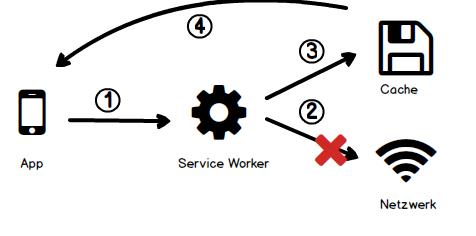
\includegraphics[width=0.75\textwidth]{networkfirst.png}
	\caption{Netzwerk dann Cache}
	\label{fig:cachingNetworkFirst}
\end{figure}



\subsubsection{Cache dann Netzwerk}
Wie Abbildung \ref{fig:cachingCacheFirst} zeigt, wird der Request hier zuerst an den Cache weitergeleitet. Befindet sich die angefragte Datei nicht im Cache, wird die Anfrage als HTTP-Request and den Server weitergeleitet. Dies ist die bevorzugte Strategie für die meisten Requests in Offline-First Anwendungen.\autocite[Kapitel 05]{BookBuildingPWAs}.

\begin{figure}[h]
	\centering
	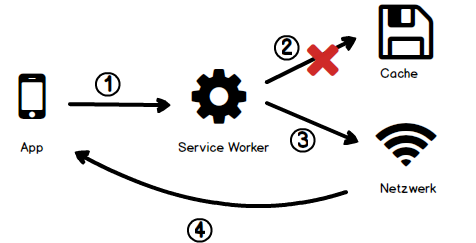
\includegraphics[width=0.75\textwidth]{cachefirst.png}
	\caption{Caching Strategie: Cache dann Netzwerk}
	\label{fig:cachingCacheFirst}
\end{figure}

\subsubsection{Nur Netzwerk}
Für Aufgaben die nur Online zu erfüllen sind, eignet sich die in Abbildung \ref{fig:cachingNetworkOnly} bezeichnete Strategie. Hier leitet der Service Worker den Request nur an das Netzwerk und nie an den Cache weiter. Offline-First Applikationen sollten so Konzipiert sein, dass diese Art Requests im Falle einer unterbrochenen Internetverbindung nachgeholt werden können, wenn der Nutzer wieder online ist.

\begin{figure}[h]
	\centering
	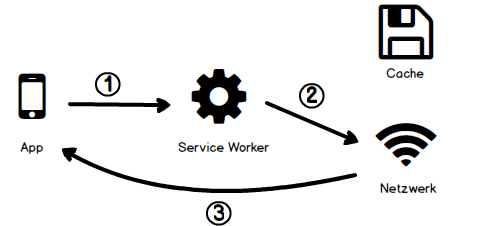
\includegraphics[width=0.75\textwidth]{networkonly.png}
	\caption{Nur Netzwerk}
	\label{fig:cachingNetworkOnly}
\end{figure}

\subsubsection{Nur Cache:}
Abbildung \ref{fig:cachingCacheOnly} zeigt, wie die angefragte Ressource nur im Cache abgefragt wird. Diese Strategie ist nur dann Sinnvoll, wenn die betroffenen Daten in einem vorherigen Schritt, beispielsweise beim Installieren des Service Workers, mit gecached wurden.

\begin{figure}[h]
	\centering
	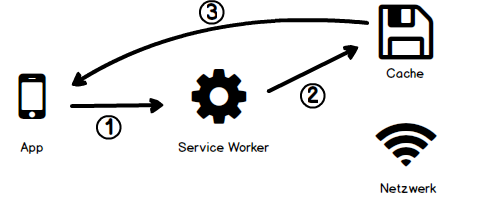
\includegraphics[width=0.75\textwidth]{cacheonly.png}
	\caption{Nur Cache}
	\label{fig:cachingCacheOnly}
\end{figure}

\section{Offline First Applikationen als verteilte Systeme}
\citet{ArticleDistributedSystems} beschreiben verteilte Systeme wie folgt: \enquote{Ein verteiltes System ist eine Sammlung von autonomen Rechenelementen, die den Benutzern als ein einziges kohärentes System erscheint.}

Die folgende Liste zeigt die Charakteristika von verteilten Systemen, zusammengefasst nach \citet{BookDistributedSystemsDefinition}.

\begin{description}
\item[Eigenständige Computer] In einem verteilten System sind mehrere eigenständige Computer zu einem System Verbunden. Diese können sich sowohl in der Hardware, also auch in der Funktionsweise unterscheiden. 
\item[Singuläres Erscheinungsbild] Für den Nutzer sind die Unterschiede zwischen den einzelnen Computern 	im System unersichtlich. Er nimmt die verteilten Computer als ein einzelnes System wahr. 
\item[Konsistente und Einheitliche Interaktion]
	Eine Konsequenz aus dem singulären Erscheinen bedeutet, dass die Interaktion des Nutzers mit dem System ist immer gleich sein sollte, unabhängig davon mit welcher Schnittstelle des Systems er tatsächlich interagiert. 
\item[Kontinuieliche Verfügbarkeit]
	Das System soll dem Nutzer kontinuierlich zur Verfügung stehen, auch wenn einzelne Teile des Systems vorübergehend ausgefallen nicht erreichbar sind.
\end{description}
	\label{tab:charakteristikaDistributedSystem}



@TODO satz einfügen Kleppnmann vortrag.
Die folgende Liste erklärt, das funktionsfähige Offline-First Applikationen die gleichen Charakteristika aufzeigen und fasst zusammen, welche Rolle diese Merkmale in der Applikation spielen.

\begin{description}		
\item[Eigenständige Computer] Der Server und verschiedene Endgeräte bilden ein System. Sobald ein Endgerät die Applikation zwischenspeichert, ist sie als eigenständiger Computer im System aktiv. Als Endgerät qualifiziert sich jedes Gerät, welches einen kompatiblen Browser betreibt, weshalb diese auch untereinander über unterschiedlichste Hardware verfügen können.
\item[Singuläres Erscheinungsbild]Die Kernfunktionalität von Offline-First Applikationen ist die Offlinefunktionalität. Offline interagiert der Nutzer nur mit seinem Endgerät, online werden die Daten gleich an den Server geschickt. Diese Unterschiede sind für den Nutzer jedoch nicht von belangen. \item[Konsistente und Einheitliche Interaktion]
Unabhängig davon, welches Endgerät der Nutzer verwendet, sollen ihm früher oder später die Änderungen aller im System aktiven Geräte angezeigt werden. Der Nutzer muss sich zu keinem Zeitpunkt Gedanken darüber machen, aus welchen Computern das System besteht.
\item[Kontinuierliche Verfügbarkeit]
Ein weiterer Aspekt, welcher sich aus der verbindlichen Offlinefunktionalität ergibt, ist die kontinuierliche Verfügbarkeit. Der Nutzer kann seine Arbeit auch fortführen wenn der Server nicht erreichbar ist. Durch SEC landen diese Änderungen früher oder später im System, wodurch die getrennte Verbindung zum Server keine Auswirkungen auf dessen Funktionsumfang hat. 
\end{description}
\label{tab:charakteristikaOfflineFirst}


Daraus schließt sich, dass es sich bei Offline-First Webanwendungen um ein verteilte Systeme handelt. Diese Erkenntnis kann dabei helfen, Probleme von Offline-First Applikationen zu lösen. Bei Offline-First handelt es sich um ein relativ junges Konzept. Obwohl Progressive Web Apps mittlerweile häufig im Netz anzutreffen sind, erfüllt deren Offlinefunktionalität selten Offline-First Kriterien. Für Probleme wie die in \ref{Problemfeld} beschriebene Synchronisation von Daten gibt es deshalb wenige beschriebene Lösungsansätze oder konkrete wissenschaftliche Arbeiten (Siehe \ref{Verwandte Arbeiten}). Mit verteilten Systemen hingegen beschäftigt sich die Informatik bereits seit den 70er Jahren \autocite{Andrews1999FoundationsOM}. Lösungen, welche für die Herausforderungen von verteilten Systemen entwickelt wurden, kommen also auch für Offline-First Webapplikationen in Frage. Eine dieser Lösungen ist die Nutzung von optimistischen Replikationsverfahren. 

\subsection{Optimistische Replikation und Eventual Consistency}

Eine der wichtigsten Grundlagen verteilter Systeme ist die Replikation von Daten. \autocite{BookDistributedSystemsConceptsAndDesign}. Datenreplikation beschreibt das Verwalten mehrerer Datenspeicher, genannt Replikationen. Diese Replikationen halten die gleichen Daten, befinden sich jedoch auf unterschiedlichen Computern\autocite{ArticleOptimisticReplication} In verteilten Systemen trägt diese Technik entscheidend dazu bei, sowohl kontinuierliche Verfügbarkeit, als auch konsistente Interaktion, beschrieben in \ref{tab:charakteristikaDistributedSystem}, zu garantieren. 


\section{CRDTs}


\subsection{Strong Eventual Consistency}
CRDTs sind Datentypen, welche in Systemen eingesetzt werden können welche dem Modell der Strong Eventual Consistency folgen. Sie werden speziell so modelliert, dass das Zusammenfuhren der Daten kommutativ, assoziativ und idempotent Erfolgen kann.


\subsection{Register}
\subsection{Counter}
\subsection{Grow-Only Set}
\section{Hybrid-Logical Clocks}

\newpage
\printbibliography



\end{document}]


